\begin{figure}[t]
  \centering
  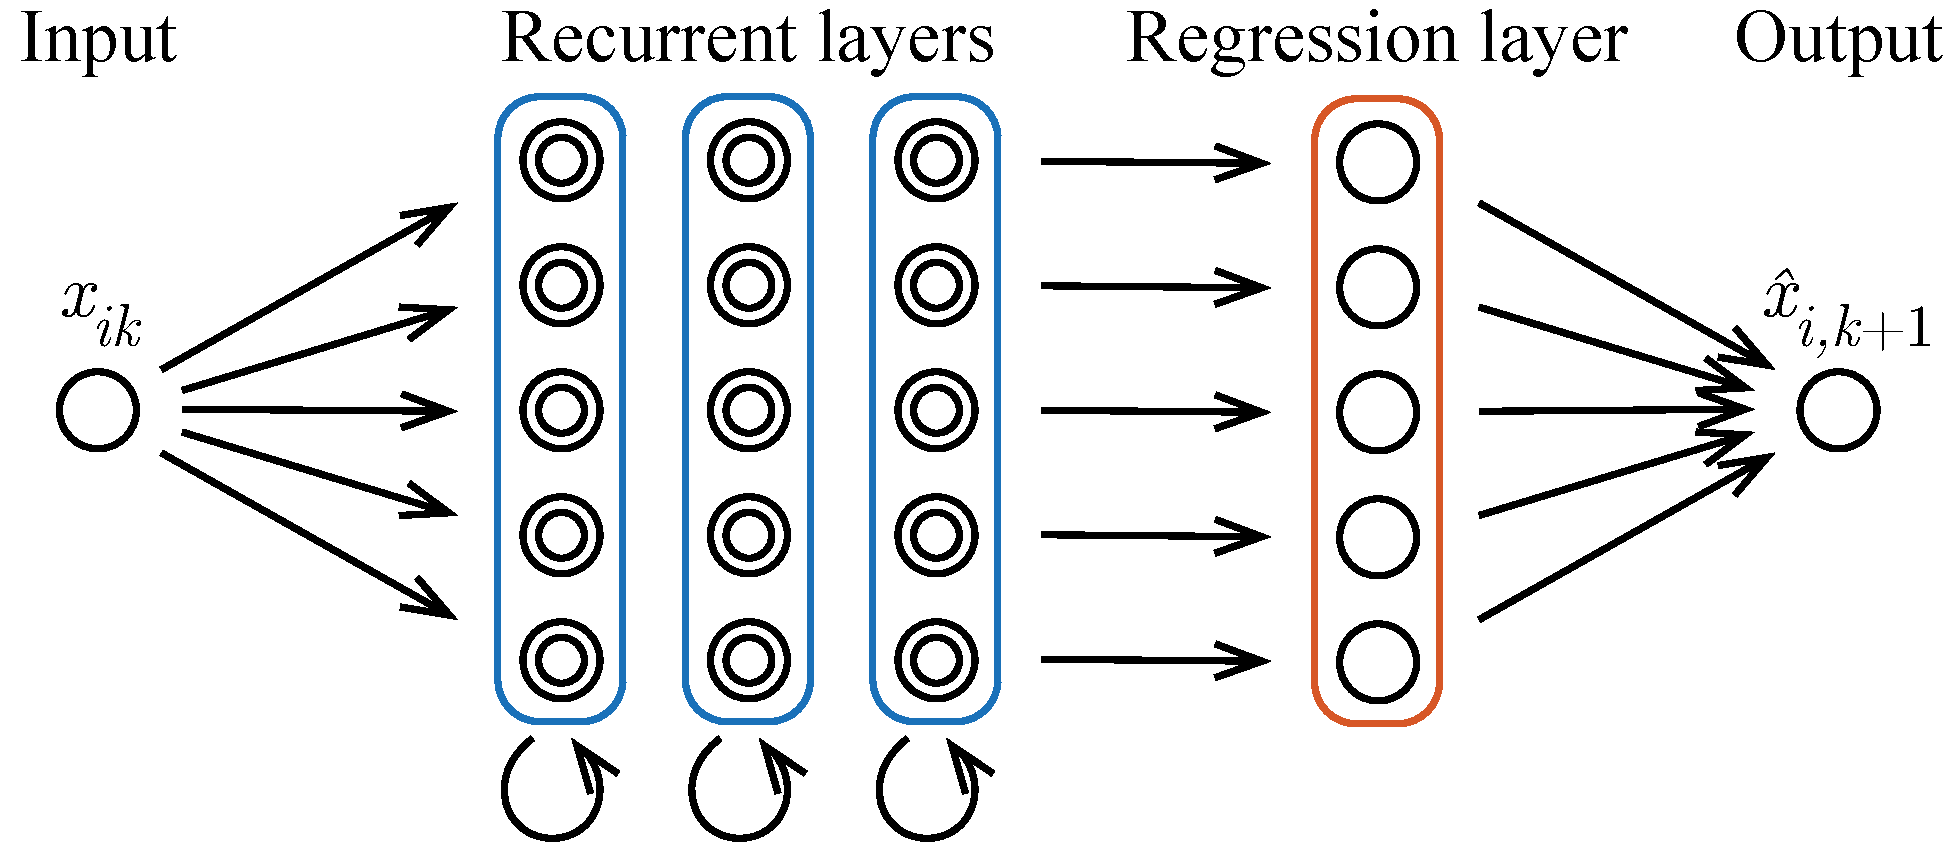
\includegraphics[width=1.0\columnwidth]{include/assets/figures/model.pdf}
  \caption{A schematic representation of our predictive model.}
  \vspace{-1.5em}
  \flab{model}
\end{figure}

As mentioned in \sref{introduction} and \sref{problem}, a part of our goal is to
assess the applicability of the latest advancements in neural networks
\cite{goodfellow2016} to modeling and prediction of fine-grained resource-usage
data. The architectures of neural networks are very diverse: one network can be
nothing like another. Since the data that we study are inherently sequential, it
is natural to found our model on the basis of recurrent neural networks
\cite{goodfellow2016}, which are specifically designed for such cases as ours.

A schematic representation of our model can be seen in \fref{model}; many of the
actual connections between the model's parts are simplified or not shown at all
in order to make the figure legible. Let us now we describe each part in detail.

\subsection{Input and Output}
The input to the model is a single $d$-dimensional data point, which can be seen
on the left-hand side of \fref{model}. Similarly, the output is a single
$d$-dimensional data point, which is depicted on the right-hand side of
\fref{model}. The input $x_{ik}$ is the value of the resource usage of an
individual task at step $k$, and the output $\hat{x}_{i,k + 1}$ is a
one-step-ahead prediction of the usage.

In order to have a long-range prediction (multiple steps ahead), we use
refeeding: the predicted value $\hat{x}_{i,k + 1}$ is fed into the model as if
it was the actual resource usage $x_{i,k + 1}$ at step $k + 1$, which is not
yet known at time step $k$. The process continues until all the desired $h$
future values are estimated.

\subsection{Recurrent Layers}
The core of the model is formed by a number of recurrent layers, which are
represented by a group of blue boxes in \fref{model}. The network can be made as
many layers deep as needed. Each layer, which is also referred to as a cell, is
composed of a number of units, which are the smallest processing elements. The
key characteristic of a unit is that it has internal memory.

There are different types of units; each one defines how a unit lets data flow
through it and updates its memory. One notable type is called \up{LSTM}
\cite{hochreiter1997}, which stands for \emph{long short-term memory}. It has
been designed to overcome the problems of traditional recurrent networks---such
as vanishing gradient when training---and it is now one of the most widely used
types. The recurrent layers of our model are \up{LSTM} cells.

In addition, each cell is enhanced with a dropout mechanism \cite{zaremba2014}.
This mechanism gives control over the regularization of the model and is there
to prevent potential overfitting.

\subsection{Fully Connected Layer}
She sells seashells on the seashore.
